\chapter{Additional Output Quantities}

\section{Black Hole Accretion}\index{black holes!supermassive}\index{black holes!accretion}\index{black holes!jets}

Properties associated with accretion onto supermassive black holes can be output by setting {\normalfont \ttfamily blackHoleOutputAccretion}$=${\normalfont \ttfamily true}. Currently, two additional properties are output for each node when this option is selected:
\begin{description}
\item[{\normalfont \ttfamily blackHoleAccretionRate}] The rate at which the supermassive black hole is accreting mass in $M_\odot$ Gyr$^{-1}$;
\item[{\normalfont \ttfamily blackHoleJetPower}] The power being emitted into jets by the black hole/accretion disk system in $M_\odot$ km$^2$ s$^{-2}$ Gyr$^{-1}$.
\end{description}

\section{Cooling Data}\index{cooling}\index{cooling!output}\index{cooling!radius}\index{cooling!rate}

Properties associated with cooling in hot halos can be output by setting {\normalfont \ttfamily hotHaloOutputCooling}$=${\normalfont \ttfamily true}. Currently, two additional properties are output for each node when this option is selected:
\begin{description}
\item[{\normalfont \ttfamily hotHaloCoolingRate}] The rate at which gas is cooling from the halo (assuming no sources of heating) in $M_\odot$ Gyr$^{-1}$;
\item[{\normalfont \ttfamily hotHaloCoolingRadius}] The characteristic cooling radius in the halo in Mpc.
\end{description}

\section{Density Contrast Data}\index{density contrast}\index{density!contrast}

Properties of nodes at density contrasts other than the virial density can be output by setting {\normalfont \ttfamily [outputDensityContrastData]}$=${\normalfont \ttfamily true}. When selected, this output option requires that a list of density contrasts, $\Delta$ (defined in units of the mean density of the Universe), be given in the {\normalfont \ttfamily [outputDensityContrastValues]} input parameter. For each specified density contrast, two properties are output for each node: {\normalfont \ttfamily nodeRadius}$\Delta$ and {\normalfont \ttfamily nodeMass}$\Delta$ which give the radius enclosing a mean density contrast of $\Delta$ and the mass enclosed within that radius. The parameter {\normalfont \ttfamily [outputDensityContrastDataDarkOnly]} controls whether density contrasts are measured for total mass ({\normalfont \ttfamily false}) or dark matter mass only ({\normalfont \ttfamily true}). In the latter case, density contrasts are defined relative to the mean dark matter density of the Universe.

\section{Descendent Node Index}\index{descendent node}\index{node!descendent}

By setting {\normalfont \ttfamily [outputDescendentIndices]}$=${\normalfont \ttfamily true} the index of the node containing the galaxy to which each current galaxy will belong at the next output time (i.e. the \gls{forwardDescendent}) will be written to the output file. To clarify, this will be the index of the node into which the galaxy descends, or the index of a node with which it merges prior to the next output time (and if that node merges with another, the index will be of that node and so on).

Note that, to operate correctly, information about which node a given node may merge with (and when this merger will happen) must be available. This is typically available in merger trees read from file providing {\normalfont \ttfamily [treeNodeMethodSatelliteOrbit]} and {\normalfont \ttfamily [mergerTreeReadPresetMergerTimes]} are both set to {\normalfont \ttfamily true}. When using randomly assigned satellite orbits and merger times, information on when merging occurs does not exist until a node becomes a satellite. Thus, if the node becomes a satellite after the current output, but before the next output, there is no way to know which node it will belong to at the next output (in such cases, the fallback assumption is no merging).

\section{Host Node Index}\index{host node}\index{node!host}

By setting {\normalfont \ttfamily [outputHostIndices]}$=${\normalfont \ttfamily true} the index of the node which hosts each node will be output to the {\normalfont \ttfamily hostIndex} dataset. For unhosted nodes (i.e. nodes which are not subhalos), a value of $-1$ is output instead.

\section{Half-Light Radii Data}\index{mass profile!half-light radius}\index{half-light radius}

Half-light radii and masses enclosed within them can be output by setting {\normalfont \ttfamily [outputHalfLightData]}$=${\normalfont \ttfamily true}. When selected the half-light radius in each specified luminosity band is output as {\normalfont \ttfamily [halfLightRadius\{luminosityID\}]} (in Mpc), where {\normalfont \ttfamily\{luminosityID\}} is the usual luminosity identifier suffix, and the total (dark + baryonic) mass within that radius is output as {\normalfont \ttfamily [halfLightMass\{luminosityID\}]} (in $M_\odot$).

\section{Half-Mass Radii}\index{mass profile!half-mass radius}\index{half-mass radius}

Half-mass radii can be output by setting {\normalfont \ttfamily [outputHalfMassData]}$=${\normalfont \ttfamily true}. When selected the half-mass radius is output as {\normalfont \ttfamily [halfMassRadius]} (in Mpc).

\section{Halo Model Quantities}\label{sec:HaloModelOutput}\index{halo model}\index{clustering!halo model}

The following quantities related to galaxy clustering are output if {\normalfont \ttfamily [outputHaloModelData]} is set to true:
\begin{description}
 \item [{\normalfont \ttfamily nodeBias}] The large scale, lineary theory bias for each node. For satellite nodes, this corresponds to the bias of their host halo;
 \item [{\normalfont \ttfamily isolatedHostIndex}] The index of the isolated node in which this node lives. This is identical to {\normalfont \ttfamily nodeIndex} for non-satellite nodes.
\end{description}
In addition to these quantities output for each node, setting {\normalfont \ttfamily [outputHaloModelData]}$=${\normalfont \ttfamily true} causes the creation of a {\normalfont \ttfamily haloModel} group in the \glc\ output file. This group contains the following:
\begin{description}
 \item [{\normalfont \ttfamily wavenumber}] A dataset giving the wavenumbers (in units of Mpc$^{-1}$) at which all output power spectra are tabulated. The minimum and maximum wavenumbers to tabulate are determined by the {\normalfont \ttfamily [haloModelWavenumberMinimum]} and {\normalfont \ttfamily [haloModelWavenumberMaximum]} parameters respectively, while the number of points to tabulate in each decade of wavenumber is determined by the {\normalfont \ttfamily [haloModelWavenumberPointsPerDecade]} parameter.
 \item [{\normalfont \ttfamily powerSpectrum}] A dataset giving the linear theory power spectrum (in units of Mpc$^3$ normalized to $z=0$ at each wavenumber specified in the {\normalfont \ttfamily wavenumber} dataset.
 \item [{\normalfont \ttfamily Output\{i\}/mergerTree\{j\}/fourierProfile\{k\}}] A dataset giving the Fourier transform of the dark matter halo density profile (dimensionless and normalized to unity at small wavenumber) for the node with index {\normalfont \ttfamily k} in merger tree with index {\normalfont \ttfamily j} at output number {\normalfont \ttfamily i}. Profiles are written only for nodes which are isolated, and are tabulated at the wavenumbers given in the {\normalfont \ttfamily wavenumber} group. Note that wavenumbers are assumed to be comoving.
\end{description}
Finally, each numbered output group is given two additional attributes, {\normalfont \ttfamily linearGrowthFactor} and {\normalfont \ttfamily linearGrowthFactorLogDerivative} which give the growth factor, $D$, and its logarithmic derivative, $\d \ln D / \d \ln a$ at the output time.

The information output can be used to construct galaxy power spectra and correlation functions.

\section{Lightcone Coordinates}\label{sec:OutputLightcone}\index{lightcones}

The position (and velocity and redshift) of a galaxy within a lightcone will be output if the parameter {\normalfont \ttfamily [outputLightconeData]}$=${\normalfont \ttfamily true}. In such cases, the following properties will be output for all galaxies:
\begin{description}
 \item [{\normalfont \ttfamily lightconePositionX}] Position of the galaxy (in comoving Mpc) along the radial direction of the lightcone;
 \item [{\normalfont \ttfamily lightconePositionY}] Position of the galaxy (in comoving Mpc) along the 1$^\mathrm{st}$ angular direction of the lightcone;
 \item [{\normalfont \ttfamily lightconePositionZ}] Position of the galaxy (in comoving Mpc) along the 2$^\mathrm{nd}$ angular direction of the lightcone;
 \item [{\normalfont \ttfamily lightconeVelocityX}] Velocity of the galaxy (in km/s) along the radial direction of the lightcone;
 \item [{\normalfont \ttfamily lightconeVelocityY}] Velocity of the galaxy (in km/s) along the 1$^\mathrm{st}$ angular direction of the lightcone;
 \item [{\normalfont \ttfamily lightconeVelocityZ}] Velocity of the galaxy (in km/s) along the 2$^\mathrm{nd}$ angular direction of the lightcone;
 \item [{\normalfont \ttfamily lightconeRedshift}] Redshift of the galaxy in the lightcone\footnote{Note that this will not, in general, be precisely the same as the redshift corresponding to the output time.};
 \item [{\normalfont \ttfamily angularWeight}] The mean number density of this galaxy per unit area on the sky (in degrees$^{-2}$). 
\end{description}
In order to allow this output a lightcone geometry must be specified, see \S\ref{sec:methodsGeometryLightcone}.

\section{Main Branch Evolution}\index{main branch!evolution}\index{evolution!main branch}

The evolution of main branch galaxies can be recorded by setting {\normalfont \ttfamily [timestepRecordEvolution]}$=${\normalfont \ttfamily true}. When set, the evolution of each main branch galaxy will be recorded at a set of {\normalfont \ttfamily [timestepRecordEvolutionSteps]} timesteps spaced logarithmically in cosmic time between {\normalfont \ttfamily [timestepRecordEvolutionBegin]} and \newline {\normalfont \ttfamily [timestepRecordEvolutionEnd]}. 

This recorded evolution will be written to the group {\normalfont \ttfamily mainProgenitorEvolution} in the \glc\ output file. Within that group two datasets, {\normalfont \ttfamily time} and {\normalfont \ttfamily expansionFactor}, give the times and expansion factors at which evolution was recorded. Then for each merger tree two datasets, {\normalfont \ttfamily stellarMass<N>} and {\normalfont \ttfamily totalMass<N>} (where {\normalfont \ttfamily <N>} is the merger tree index), give the stellar and total baryonic mass of the main branch progenitor at each timestep.

\section{Main Branch Status}\index{merger trees!main branch}

The status of each node with respect to the main branch of its merger tree can be output by setting {\normalfont \ttfamily [outputMainBranchStatus]}$=${\normalfont \ttfamily true}. When set, the status will be output as {\normalfont \ttfamily nodeIsOnMainBranch}, with a value of 1 indicating that the node is a primary progenitor of the final halo (i.e. is on the main branch of the tree) and a value of 0 indicating that it is not.

\section{Mass Profile Data}\index{mass profile}

Masses enclosed within specific radii can be output by setting {\normalfont \ttfamily [outputMassProfileData]}$=${\normalfont \ttfamily true}. When selected, this output option requires that a list of radii, $r$ (in Mpc), be given in the {\normalfont \ttfamily [outputMassProfileRadii]} input parameter. For each specified radius, the total (dark + baryonic) mass will be output as {\normalfont \ttfamily massProfile}$r$.

\section{Merger Tree Links and Node Isolation}\index{merger tree!links}\index{galaxies!satellite}\index{galaxies!central}\index{nodes!isolated}\index{nodes!substructure}

The following properties are output to permit the merger tree structure to be recovered:
\begin{description}
 \item [{\normalfont \ttfamily nodeIndex}] A unique\footnote{Node indices are typically unique, but there is no actual requirement within \protect\glc\ that this must be the case. A merger tree construction method could create nodes with non-unique indices.} (within a tree) integer index identifying the node;
 \item [{\normalfont \ttfamily parentIndex}] The index of this node's parent node (or $-1$ if it has no parent);
 \item [{\normalfont \ttfamily siblingIndex}] The index of this node's sibling node (or $-1$ if it has no sibling);
 \item [{\normalfont \ttfamily satelliteIndex}] The index of this node's first satellite node (or $-1$ if it has no satellites);
 \item [{\normalfont \ttfamily nodeIsIsolated}] Will be $0$ for a node which is a subhalo inside some other node (i.e. a satellite galaxy\index{satellite galaxies!identifying}) or $1$ for a node that is an isolated halo (i.e. a central galaxy\index{central galaxies!identifying}).
\end{description}

The {\normalfont \ttfamily nodeIndex} property corresponds by default to the index of the node in the original merger tree. This means that as a galaxy evovles through the tree and, in particular, gets promoted into a new halo the index associated with a galaxy will change. This is useful to identify where the galaxy resides in the original (unevolved) tree structure, but does not allow galaxies to be traced from one output to the next using their {\normalfont \ttfamily nodeIndex} value. By setting {\normalfont \ttfamily [nodePromotionIndexShift]}$=${\normalfont \ttfamily true} this behavior can be changed such that the value of {\normalfont \ttfamily nodeIndex} will reflect the index of the earliest progenitor node along the main branch of the current node. As such, this index will remain the same for a given galaxy during its evolution\index{galaxies!tracing through outputs}\index{galaxies!indices}\index{nodes!indices}\index{indices!nodes}\index{indices!galaxies}. These two alternative algorithms for propagating node indices are illustrated in Figure~\ref{fig:NodePromotionIndexAlgorithms}.

\begin{figure}
 \begin{center}
 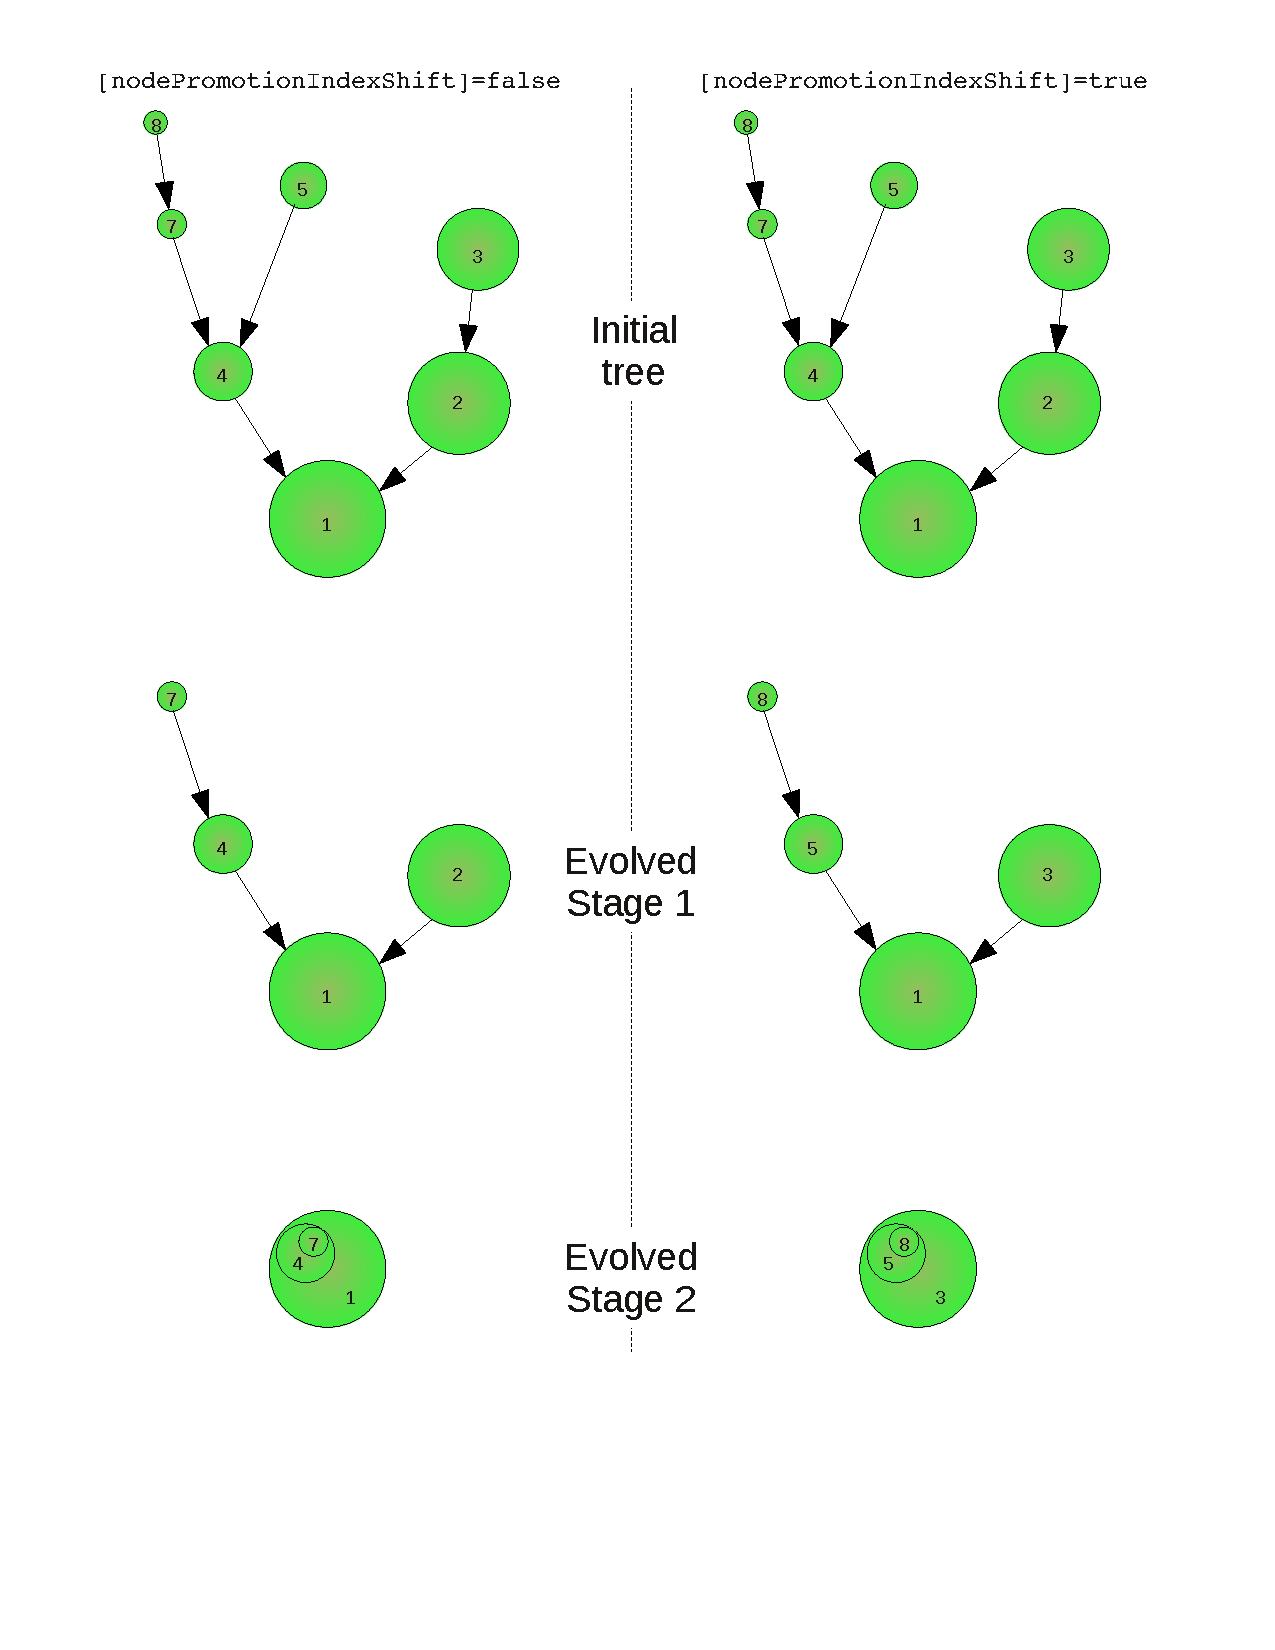
\includegraphics[width=140mm]{Diagrams/NodePromotionIndices.pdf}
 \end{center}
 \caption{Illustration of options for the propagation of node indices during node promotion events. Two identical trees (top row) are evolved with {\normalfont \ttfamily [nodePromotionIndexShift]}$=${\normalfont \ttfamily false} (left column) and {\normalfont \ttfamily [nodePromotionIndexShift]}$=${\normalfont \ttfamily true} (right column). The middle and lower rows indicate the resulting node indices after two stages of tree evolution.}
 \label{fig:NodePromotionIndexAlgorithms}
\end{figure}

\section{Merger Tree Data for Rendering}\index{merger tree!rendering}

Data on the structure of a merger tree and its halos useful for rendering the tree as a 3-D structure can be output using the \hyperlink{merger_trees.render.F90:merger_trees_render}{\normalfont \ttfamily Merger\_Trees\_Render} module. Calling \hyperlink{merger_trees.render.F90:merger_trees_render:merger_trees_render_dump}{\normalfont \ttfamily Merger\_Trees\_Render\_Dump} with a tree as the only argument will cause the tree structure will be dumped to a file named {\normalfont \ttfamily render\_$\langle$treeIndex$\rangle$\_$\langle$outputIndex$\rangle$.hdf5} where $\langle${\normalfont \ttfamily treeIndex}$\rangle$ is the index of the tree and $\langle${\normalfont \ttfamily outputIndex}$\rangle$ is an incremental counter that tracks the number of outputs for this tree. The output is a simple HDF5 file containing the following datasets:
\begin{description}
 \item [{\normalfont \ttfamily nodeIndex}] Index of the node;
 \item [{\normalfont \ttfamily parentIndex}] Index of the parent node;
 \item [{\normalfont \ttfamily childIndex}] Index of the child node;
 \item [{\normalfont \ttfamily time}] Time of the node;
 \item [{\normalfont \ttfamily expansionFactor}] Corresponding expansion factor;
 \item [{\normalfont \ttfamily radiusVirial}] Virial radius of the node;
 \item [{\normalfont \ttfamily position}] $(x,y,z)$ position of the node.
\end{description}

\section{Merger Tree Structure}\index{merger tree!structure}

The structure of each merger tree can optionally be dumped to a file suitable for post-processing with \href{http://www.graphviz.org/}{\normalfont \scshape dot} after every step of evolution. To request this output set {\normalfont \ttfamily [mergerTreesDumpStructure]}$=${\normalfont \ttfamily true}. After each evolution step the tree structure will be dumped to a file named {\normalfont \ttfamily mergerTreeDump:$\langle$treeIndex$\rangle$:$\langle$outputIndex$\rangle$.gv} where $\langle${\normalfont \ttfamily treeIndex}$\rangle$ is the index of the tree and $\langle${\normalfont \ttfamily outputIndex}$\rangle$ is an incremental counter that tracks the number of outputs for this tree. These files can be processed with \href{http://www.graphviz.org/}{\normalfont \scshape dot} to produce a diagram of the tree structure. The node currently being evolved will be highlighted in green. This output option makes use of the \hyperlink{objects.merger_trees.dump.F90:merger_trees_dump}{\normalfont \ttfamily Merger\_Trees\_Dump} module to create the outputs.

\section{Most Massive Progenitor}

Setting {\normalfont \ttfamily [outputMostMassiveProgenitor]}$=${\normalfont \ttfamily true} causes the property {\normalfont \ttfamily isMostMassiveProgenitor} to be output. This property will be $1$ for the most massive progenitor node in a tree at each output time and $0$ for all other nodes.

\section{Projected Density}\index{projected density!outputting}\index{outputs!projected density}

Setting {\normalfont \ttfamily [outputProjectedDensityData]}$=${\normalfont \ttfamily true} causes the projected density of the node to be output at specified radii. The radii and types of projected density to output is specified by the {\normalfont \ttfamily outputProjectedDensityRadii} parameter. This parameter's value can contain multiple entries. Each entry is of the form:
\begin{verbatim}
  radiusType:componentType:massType:loading?:radius
\end{verbatim}
The elements of this colon-separated specifier determine the radius at which the projected density is computed, which components/mass types should be counted, and whether baryonic loading of the halo should be accounted for. The elements have the following meaning:
\begin{description}
 \item [{\normalfont \ttfamily radius}] the numerical value of the radius at which to compute the projected density (with units specified by the {\normalfont \ttfamily radiusType} element);
 \item [{\normalfont \ttfamily radiusType}] specifies the units of the {\normalfont \ttfamily radius} element---valid options are {\normalfont \ttfamily diskRadius}, {\normalfont \ttfamily diskHalfMassRadius}, {\normalfont \ttfamily spheroidRadius}, {\normalfont \ttfamily spheroidHalfMassRadius}, {\normalfont \ttfamily darkMatterScaleRadius}, {\normalfont \ttfamily virialRadius}, just {\normalfont \ttfamily radius} (which implies radii are given in units of Mpc), {\normalfont \ttfamily galacticMassFraction\{\textless fraction\textgreater\}}, or \newline {\normalfont \ttfamily galacticLightFraction\{\textless fraction\textgreater\}\{\textless luminosity\textgreater\}}, where the final two form specify a radius containing a fixed {\normalfont \ttfamily \textless fraction\textgreater} of the galactic mass or light respectively (for the case of galactic light, {\normalfont \ttfamily \textless luminosity\textgreater} specifies the band, e.g. {\normalfont \ttfamily SDSS\_r:rest:z0.0000});
 \item [{\normalfont \ttfamily componentType}] specifies which components of the node should be counted---allowed values are {\normalfont \ttfamily all}, {\normalfont \ttfamily disk}, {\normalfont \ttfamily spheroid}, {\normalfont \ttfamily hotHalo}, {\normalfont \ttfamily darkHalo}, and {\normalfont \ttfamily blackHole};
 \item [{\normalfont \ttfamily massType}] specifies which types of mass should be counted---allowed values are {\normalfont \ttfamily all}, {\normalfont \ttfamily dark}, {\normalfont \ttfamily baryonic}, {\normalfont \ttfamily galactic}, {\normalfont \ttfamily gaseous}, {\normalfont \ttfamily stellar}, and {\normalfont \ttfamily blackHole};
 \item [{\normalfont \ttfamily loading?}] option should be either {\normalfont \ttfamily loaded} or {\normalfont \ttfamily unloaded}, and specifies whether the effect of baryonic loading (i.e. adiabatic contraction) should be included in the calculation of the projected density.
\end{description}

\section{Rotation Curve}\index{rotation curve!outputting}\index{outputs!rotation curve}

Setting {\normalfont \ttfamily [outputRotationCurveData]}$=${\normalfont \ttfamily true} causes the rotation curve of the node to be output at specified radii. The radii and types of rotation curve to output is specified by the {\normalfont \ttfamily outputRotationCurveRadii} parameter. This parameter's value can contain multiple entries. Each entry is of the form:
\begin{verbatim}
  radiusType:componentType:massType:loading?:radius
\end{verbatim}
The elements of this colon-separated specifier determine the radius at which the rotation curve is computed, which components/mass types should be counted, and whether baryonic loading of the halo should be accounted for. The elements have the following meaning:
\begin{description}
 \item [{\normalfont \ttfamily radius}] the numerical value of the radius at which to compute the rotation curve (with units specified by the {\normalfont \ttfamily radiusType} element);
 \item [{\normalfont \ttfamily radiusType}] specifies the units of the {\normalfont \ttfamily radius} element---valid options are {\normalfont \ttfamily diskRadius}, {\normalfont \ttfamily diskHalfMassRadius}, {\normalfont \ttfamily spheroidRadius}, {\normalfont \ttfamily spheroidHalfMassRadius}, {\normalfont \ttfamily darkMatterScaleRadius}, {\normalfont \ttfamily virialRadius}, just {\normalfont \ttfamily radius} (which implies radii are given in units of Mpc), {\normalfont \ttfamily galacticMassFraction\{\textless fraction\textgreater\}}, or \newline {\normalfont \ttfamily galacticLightFraction\{\textless fraction\textgreater\}\{\textless luminosity\textgreater\}}, where the final two form specify a radius containing a fixed {\normalfont \ttfamily \textless fraction\textgreater} of the galactic mass or light respectively (for the case of galactic light, {\normalfont \ttfamily \textless luminosity\textgreater} specifies the band, e.g. {\normalfont \ttfamily SDSS\_r:rest:z0.0000});
 \item [{\normalfont \ttfamily componentType}] specifies which components of the node should be counted---allowed values are {\normalfont \ttfamily all}, {\normalfont \ttfamily disk}, {\normalfont \ttfamily spheroid}, {\normalfont \ttfamily hotHalo}, {\normalfont \ttfamily darkHalo}, and {\normalfont \ttfamily blackHole};
 \item [{\normalfont \ttfamily massType}] specifies which types of mass should be counted---allowed values are {\normalfont \ttfamily all}, {\normalfont \ttfamily dark}, {\normalfont \ttfamily baryonic}, {\normalfont \ttfamily galactic}, {\normalfont \ttfamily gaseous}, {\normalfont \ttfamily stellar}, and {\normalfont \ttfamily blackHole};
 \item [{\normalfont \ttfamily loading?}] option should be either {\normalfont \ttfamily loaded} or {\normalfont \ttfamily unloaded}, and specifies whether the effect of baryonic loading (i.e. adiabatic contraction) should be included in the calculation of the rotation curve.
\end{description}

\section{Satellite Mergers}\index{satellite!mergers!outputting}\index{mergers!satellite!outputting}

Setting {\normalfont \ttfamily [outputSatelliteMergers]} to {\normalfont \ttfamily true} will cause data to be output for each satellite merger event. Data is stored to datasets in the {\normalfont \ttfamily satelliteMergers} group. Datasets output are:
\begin{description}
\item{\normalfont \ttfamily [indexHost]} the index of the host halo in the merger;
\item{\normalfont \ttfamily [indexSatellite]} the index of the satellite halo in the merger;
\item{\normalfont \ttfamily [indexTree]} the index of the merger tree in which the merger occurred;
\item{\normalfont \ttfamily [massHost]} the mass of the host halo;
\item{\normalfont \ttfamily [massSatellite]} the mass of the satellite halo;
\item{\normalfont \ttfamily [time]} the time at which the merger occurred.
\end{description}

\section{Satellite Orbital Pericenter}\index{satellite!orbit!outputting}\index{orbits!satellite!outputting}

Setting {\normalfont \ttfamily [outputSatellitePericenterData]} to {\normalfont \ttfamily true} will cause the pericentric values of the radius and velocity of each satellite node's orbit to be output as {\normalfont \ttfamily satellitePericenterRadius} and {\normalfont \ttfamily satellitePericenterVelocity} respectively.

\section{Star Formation Rates}\index{star formation rate!outputting}\index{outputs!star formation rate}

By default the star formation rate in each galaxy is \emph{not} output. However, setting {\normalfont \ttfamily [diskOutputStarFormationRate]} to true will cause the current star formation rate in the disk of each galaxy to be output as {\normalfont \ttfamily diskStarFormationRate} (in units of $M_\odot$/Gyr). The {\normalfont \ttfamily [spheroidOutputStarFormationRate]} has the same effect for the spheroid component.

\section{Velocity Dispersion}\index{velocity dispersion!outputting}\index{outputs!velocity dispersion}

Setting {\normalfont \ttfamily [outputVelocityDispersionData]}$=${\normalfont \ttfamily true} causes the velocity dispersion of the node to be output at specified radii, for specified components. The radii, components and type of velocity dispersion to output are specified by the {\normalfont \ttfamily outputVelocityDispersionRadii} parameter. This parameter's value can contain multiple entries. Each entry is of the form:
\begin{verbatim}
  radiusType:componentType:massType:loading?:direction:radius
\end{verbatim}
The elements of this colon-separated specifier determine the radius at which the velocity dispersion is computed, which component/mass type the velocity dispersion should be computed for, whether baryonic loading of the halo should be accounted for, and for which direction the velocity dispersion should be computed. The elements have the following meaning:
\begin{description}
 \item [{\normalfont \ttfamily radius}] the numerical value of the radius at which to compute the velocity dispersion (with units specified by the {\normalfont \ttfamily radiusType} element);
 \item [{\normalfont \ttfamily radiusType}] specifies the units of the {\normalfont \ttfamily radius} element---valid options are {\normalfont \ttfamily diskRadius}, {\normalfont \ttfamily diskHalfMassRadius}, {\normalfont \ttfamily spheroidRadius}, {\normalfont \ttfamily spheroidHalfMassRadius}, {\normalfont \ttfamily darkMatterScaleRadius}, {\normalfont \ttfamily virialRadius}, just {\normalfont \ttfamily radius} (which implies radii are given in units of Mpc), {\normalfont \ttfamily galacticMassFraction\{\textless fraction\textgreater\}}, or \newline {\normalfont \ttfamily galacticLightFraction\{\textless fraction\textgreater\}\{\textless luminosity\textgreater\}}, where the final two form specify a radius containing a fixed {\normalfont \ttfamily \textless fraction\textgreater} of the galactic mass or light respectively (for the case of galactic light, {\normalfont \ttfamily \textless luminosity\textgreater} specifies the band, e.g. {\normalfont \ttfamily SDSS\_r:rest:z0.0000});
 \item [{\normalfont \ttfamily componentType}] specifies which component of the node the velocity dispersion should be computed for---allowed values are {\normalfont \ttfamily all}, {\normalfont \ttfamily disk}, {\normalfont \ttfamily spheroid}, {\normalfont \ttfamily hotHalo}, {\normalfont \ttfamily darkHalo}, and {\normalfont \ttfamily blackHole}\footnote{Note that attempting to compute the velocity dispersion for a black hole or disk for example won't make any sense.};
 \item [{\normalfont \ttfamily massType}] specifies which type of mass the velocity dispersion should be computed for---allowed values are {\normalfont \ttfamily all}, {\normalfont \ttfamily dark}, {\normalfont \ttfamily baryonic}, {\normalfont \ttfamily galactic}, {\normalfont \ttfamily gaseous}, {\normalfont \ttfamily stellar}, and {\normalfont \ttfamily blackHole};
 \item [{\normalfont \ttfamily loading?}] option should be either {\normalfont \ttfamily loaded} or {\normalfont \ttfamily unloaded}, and specifies whether the effect of baryonic loading (i.e. adiabatic contraction) should be included in the calculation of the velocity dispersion;
 \item [{\normalfont \ttfamily direction}] should be one of {\normalfont \ttfamily radial} (computes the radial component of velocity dispersion), {\normalfont \ttfamily lineOfSight\{\textless luminosity\textgreater\}} (computes the line-of-sight velocity dispersion), {\normalfont \ttfamily lineOfSightInteriorAverage\{\textless luminosity\textgreater\}} (computes the line-of-sight velocity dispersion averaged interior to the given radius), or {\normalfont \ttfamily lambdaR\{\textless luminosity\textgreater\}} (computes the $\lambda_\mathrm{R}$ statistic of \citealt{cappellari_sauron_2007})---in the latter three cases {\normalfont \ttfamily \{\textless luminosity\textgreater\}} specifies which band should be used to weight the velocity dispersion, alternatively setting {\normalfont \ttfamily \{\textless luminosity\textgreater\}}$=${\normalfont \ttfamily mass} (or just leaving off this specifier entirely) will use mass weighting instead.
\end{description}

\section{Virial Quantities}\index{virial}

The following quantities related to the virialized region of each node are output if {\normalfont \ttfamily outputVirialData} is set to true:
\begin{description}
 \item [{\normalfont \ttfamily nodeVirialRadius}] The virial radius (following whatever definition of virial overdensity was selected in \glc) in units of Mpc;
 \item [{\normalfont \ttfamily nodeVirialVelocity}] The circular velocity at the virial radius (in km/s).
\end{description}
